\documentclass[12pt]{article}

 \usepackage{color}
\usepackage[portuguese]{babel}
\usepackage[utf8]{inputenc}
\usepackage{indentfirst}
\usepackage{graphicx}
\usepackage{verbatim}
\usepackage{listings}
\usepackage{url}
\usepackage{stringenc}
\usepackage{pdfescape}
 \usepackage{subfig}
\begin{document}

\setlength{\textwidth}{16cm}
\setlength{\textheight}{22cm}
\title{\Huge\textbf{\textit{StatusUpdade}}\linebreak
\Large\textbf{2º Trabalho}\linebreak\linebreak\linebreak

\includegraphics[width=9cm]{feup.pdf}\linebreak \linebreak
\Large{Mestrado Integrado em Engenharia Informática e Computação} \linebreak
\Large{Sistemas Distribuídos - EIC0036}\linebreak
}
\author{
Gil Filipe da Rocha - 201100629\\João Pedro Matos Teixeira Dias - 201106781\\
João Carlos Teixeira de Sá - 201107925
\\Manuel João Gonçalves Vieira de Castro - 200900654
\\
 \\ Faculdade de Engenharia da Universidade do Porto \\ Rua Roberto Frias, s\/n, 4200-465 Porto, Portugal
 \vspace{1cm}}
%\date{Junho de 2007}
\maketitle
\thispagestyle{empty}

%************************************************************************************************
%************************************************************************************************

\newpage

\tableofcontents

%************************************************************************************************
%************************************************************************************************

%*************************************************************************************************
%************************************************************************************************

\newpage

\section{Introdução}

O presente relatório apresenta o trabalho desenvolvido na unidade curricular de Sistemas Distríbuidos, utilizando os conceitos apresentados na unidade, mais especificamente tirando partido do paradigma REST (\textit{Representational state transfer}) para a realização da comunicação entre uma aplicação móvel e um servidor remoto.

	A aplicação móvel desenvolvida incide sobre a atual dependência da população geral diaria de serviços baseados na \textit{web}, e também, por outro lado, da importância por parte de administradores de sistemas  de manter sobre vígia recorrente vários serviços \textit{web} pelos quais são responsáveis. Sendo assim a aplicação \textit{StatusUpdate} consegue mostrar, no momento, a disponibilidade do serviço, tempo de \textit{loading} assim como outros promenores adicionais disponibilizados pela maioria dos servidores.
	
	Também foi tirado partido da integração do Twitter na aplicação, sendo que vários serviços tem contas de \textit{status} presentes com informação bastante útil.
	
	Sendo assim, pensamos que surge assim uma aplicação com bastante  utilidade, ainda não existindo nada atualmente que desempenhe estas funções da forma apresentada, especialmente no universo móvel.
	
	De encontro a inicial proposta de trabalho apresentada, todos os tópicos foram cobertos, sendo que foram acrescentadas funcionalidades não apresentadas inicialmente mas que surgiram como úteis aquando o desenvolvimento da aplicação. 

\subsection{Divisão de trabalho e atribuição de tarefas}

Devido ao trabalho abranger duas areas especificas, o servidor e o cliente, a primeira fase de divisão de trabalho foi facilitada, sendo que foi atribuido a João Pedro Dias e a João Sá a parte do cliente, ou seja da aplicação móvel, e a Gil Rocha e João Castro a parte de servidor.  Tanto de uma parte como de outra foi despendiado tempo a aprender as novas tecnologias, neste caso MongoDB, Node.js e mesmo Windows Phone 8.1 . 

Após o início do desenvolvimento apercebemo-nos de que a implementação na parte do cliente iria ser mais complexa, e assim, numa fase em que já se encontravam as funcionalidade de login/logout de utilizadores e o armazenamento da informação relativa a cada um destes implemnetadas, tanto do lado de servidor como do lado do cliente, efetuou-se uma nova divisão do trabalho em que João Pedro Dias ficou responsável pela apresentação na aplicação de todos os serviços subscritos assim como a informação de cada um destes (\textit{GET} a vários servidores, interpretação e apresentação da informação relevante como disponíbilidade e tempo de resposta), João Sá responsável pela apresentação do \textit{feed} do Twitter usando a sua API, Gil Rocha com a continuação de implementação das funcionalidades necessárias no servidor, principalmente responsáveis pelas funcionalidades CRUD (Create, Read, Update, Delete) para cada utilizador, e João Castro por aplicar na aplicação móvel os respetivos botões necessários para estas tarefas, com as chamadas ao servidor necessárias.

Aproxima-se que foi utilizado um total de 60 horas de trabalho total, sendo que estas foram divididas entre as aulas práticas de SDIS (no total de 6 horas) e trabalho extra-aula no total de 54 horas, sendo que estas foram de forma quase de igual divididas por todos os elementos do grupo, sendo que em certas fases do trabalho foi necessário a colaboração de todos ``ao mesmo tempo'', como, por exemplo, para decidir tecnológias e a comunicação cliente-servidor. 

\section{Arquitetura e implementação}
\subsection{Tecnologias utilizadas}
	O presente projeto foi desenvolvido com base no paradigma REST, ou seja usando os métodos disponíveis no protocolo HTTP 1.1. Este paradigma é atualmente muito falado, e usando tecnologias de alta performance e recentes é uma mais valia tirar partido dele Assim sendo, para o servidor foi utilizado Node.js e com concordância com este sistema foi utilizada uma base de dados NoSQL, MongoDB. No lado da aplicação móvel esta foi desenvolvida usando a linguagem C\# sobre a plataforma móvel Windows Phone 8.1 (versão atualmente ainda em fase de desenvolvimento e disponível apenas para \textit{developers}).
	
	A escolha de se utilizar Node.js no servidor trata-se de além da fácilidade de programação graças a ser utilizada a linguagem JavaScript, a grande quantidade de módulos adicionais existentes como é o caso do \textit{expressjs} e do \textit{moongose}.	 No nosso caso o Node.js facilitou em muito a comunicação REST tanto devido a utilizaçao do módulo \textit{expressjs} e devido a todo o \textit{server-side} ser altamente escalável, e toda a comunicação ser feita assincronamente. Por outro lado a base de dados MongoDB é também altamente escalável e orientada a documentos, sendo mais fácil armazenar informação e mais flexivel. 
	
	Por outro lado, a escolha da plataforma móvel Windows Phone deveu-se a ser utilizada a linguagem C\# no seu desenvolvimento e também pelas ferramentas disponíveis para desenvolvimento, neste caso, Visual Studio 2013, que é um IDE muito mais estável e poderoso e devido a existência do repositório NuGet que disponibiliza bibliotecas de alta qualidade para váriadas situações. Acrescentando a isto, sendo que foi utilizada a versão de \textit{developer preview} do Windows Phone 8.1 possibilitou a aprendizagem das alterações relativamente a versões anteriores do Sistema Operativo, que serão a partir de agora usadas.
	
	Acrescentado, foi utilizado o serviço de hospedagem para servidores \textit{Node.js} Heroku (https://www.heroku.com/)  e o serviço de hospedagem de para a base de dados \textit{mongolab}  (https://mongolab.com/), necessitando assim de ser efetuada a ligação entre estes dois serviços.
	
\subsection{Arquitetura}	
\begin{figure}
 \centering
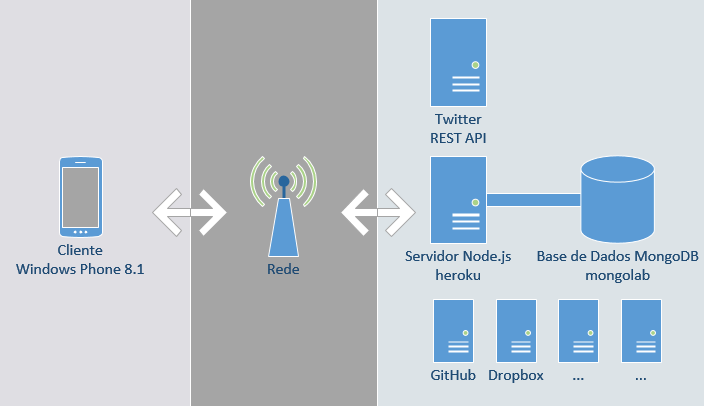
\includegraphics[scale=0.75]{rede.png}
 \caption{Esquemática do funcionamento da aplicação.}
 \label{figure:example}
\end{figure}

De acordo com o que é demonstrado na fig. 1 apresentada, o nosso sistema é dividido entre \textit{server-side} e \textit{client-side}, e além destes depende da REST API do serviço Twitter e das respostas de todos os outros servidores cujos serviços são vigiados pela aplicação (p. ex. GitHub).
	
	Essencialmente a comunicação baseia-se em pedidos POST e GET utilizados tanto para guardar informação na nossa base de dados assim como para obter informação tanto do nosso servidor assim como do Twitter e todos os restantes serviços. Acrescentando toda a comunicação efetuada é assíncrona.

\subsection{Implementação}

Toda a implentação a nível móvel foi baseada em pedidos assíncronos entre a aplicação e o nosso servidor, e também de igual forma para todos os pedidos para API e outros serviços. A correta implementação desta comunicação, evitar falhas e efetuar sempre verificações, como por exemplo, verificação intensiva do valor do \textit{Status Code}, verificou-se como sendo o mais complexo, pois a sua má estruturação levaria a recorrentes falhas nos dados apresentados ao utilizador aquando a utilização da aplicação. 

\renewcommand{\arraystretch}{1.5}
\begin{table}[h!]
\begin{tabular}{p{2cm}|p{2.5cm}|p{2.5cm}|p{2.5cm}|p{2cm}}
Resource (URI) & GET  & PUT & POST  & DELETE  \\\hline
/ & Abre \textit{server page index} &  - & - &  - \\\hline
/signup &  -& - & Cria conta de utilizador e efetua \textit{login}  &- \\\hline
/login &-  &-  & Efetua \textit{login} de utilizador & - \\\hline
/apps &  -& - & Retorna os serviços de um utilizador &-  \\\hline
/default & - & - & Retorna o Twitter de um serviço &-  \\\hline
/addsite &  -& - &Adiciona um serviço a lista por defeito &-  \\\hline
/allsites &  Retorna os serviços disponíveis por defeito &-  &- & - \\\hline
/subscribe &-  &  -&Adiciona um serviço a um utilizador& - \\\hline
/remove & - &  -& Remove um serviço de um utilizador & - \\\hline
/logout &  -& - & Termina sessão de um utilizador &-  \\\hline
\end{tabular}
\caption{API REST implementada em Node.js}
\end{table}

A nível do servidor as maiores dificuldades foram a aprendizagem a plataforma Node.js e de como seria definida a API, assim como a adicional necessidade de ser estabelecida a ligação a uma base de dados em outro seviço de forma a ser usado MongoDB. Assim numa primeira parte defenindo a RESTful API chegou-se a estrutura apresentada na tabela.


\section{Utilização} 
\begin{figure}[ht!]
\centering
\parbox{5cm}{
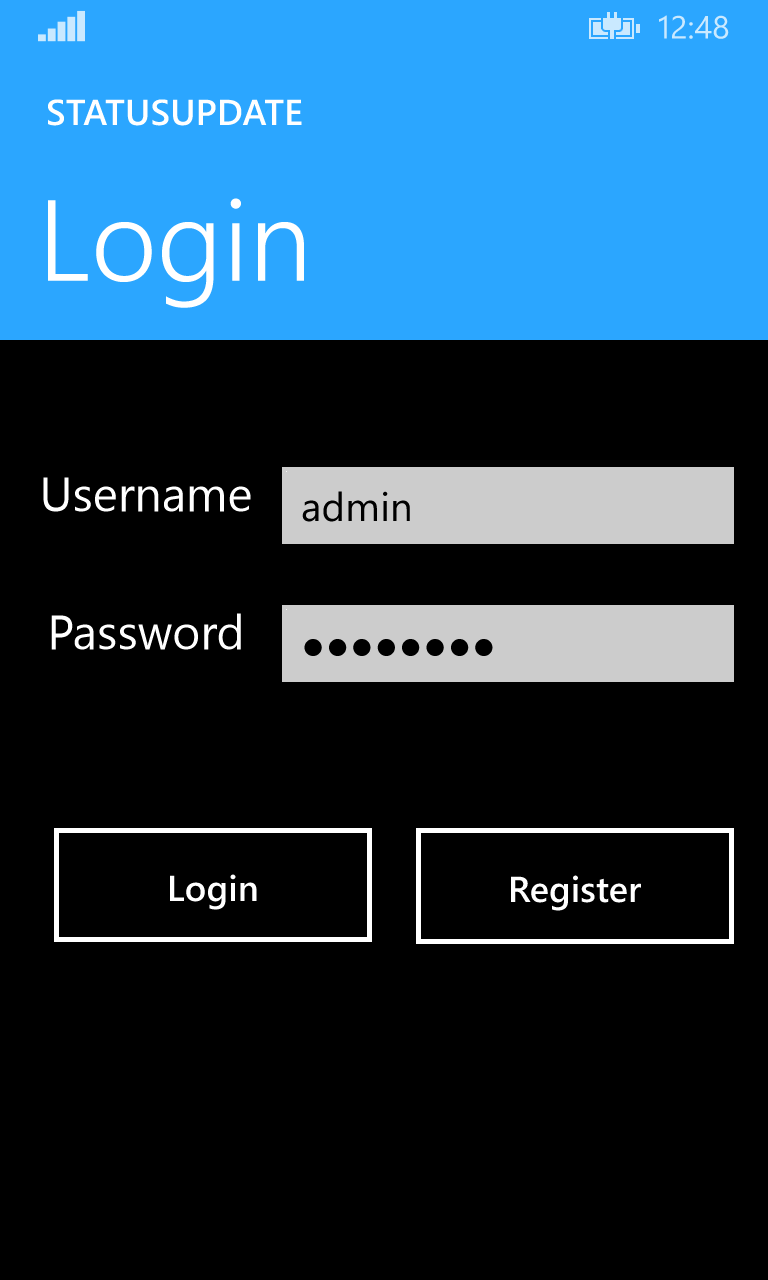
\includegraphics[width=5cm]{1.png}
\caption{Ecra inicial:  Login ou Registo na aplicação.}
}
\qquad
\begin{minipage}{5cm}
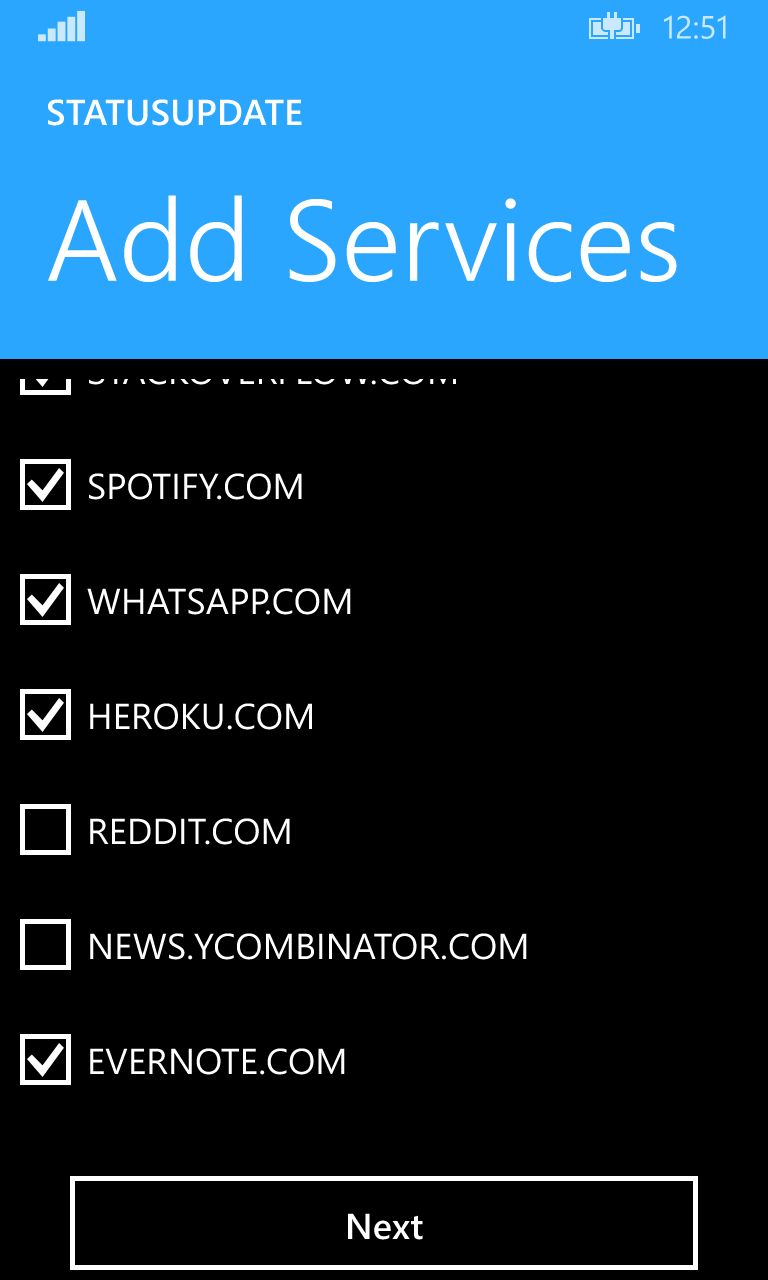
\includegraphics[width=5cm]{2.png}
\caption{Adicionar serviços: apresentado após fazer registo apenas.}
\end{minipage}
\end{figure}
\begin{figure}[ht!]
\centering
\parbox{5cm}{
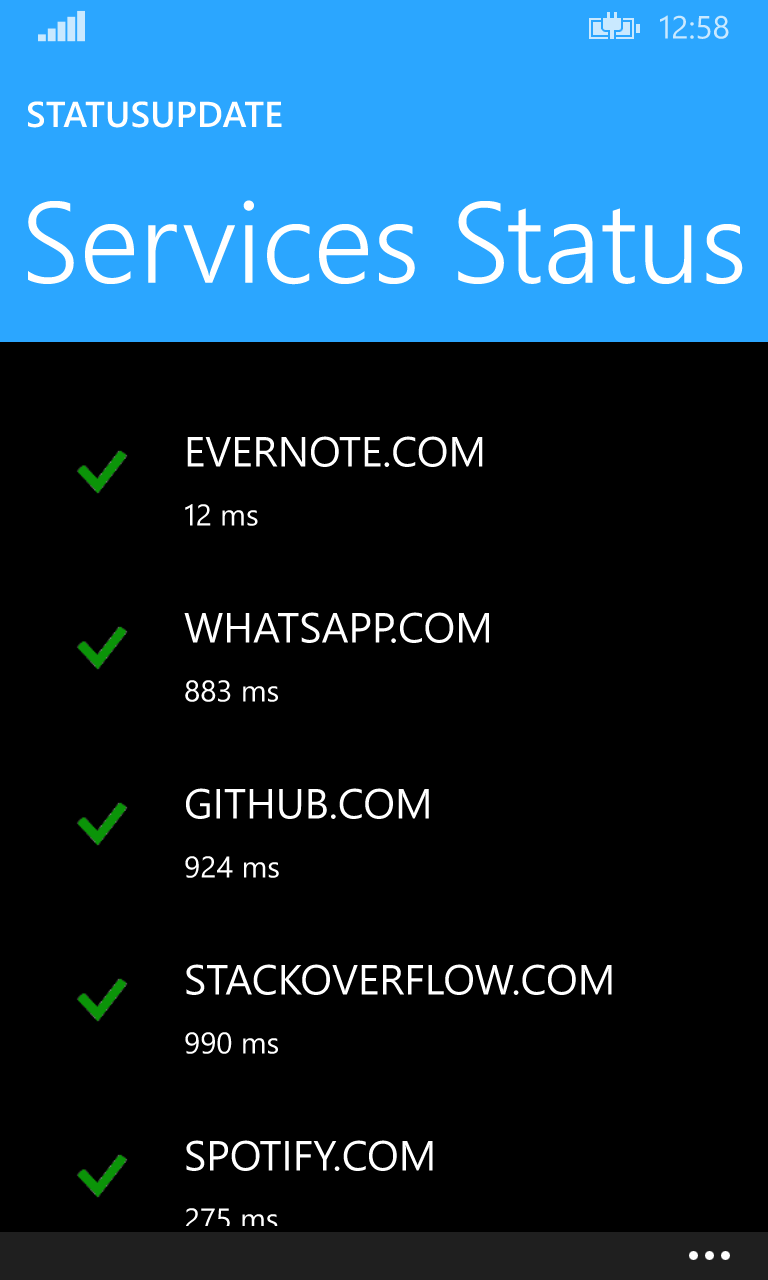
\includegraphics[width=5cm]{7.png}
\caption{Lista de serviços subscritos.}
\label{fig:2figsA}}
\qquad
\begin{minipage}{5cm}
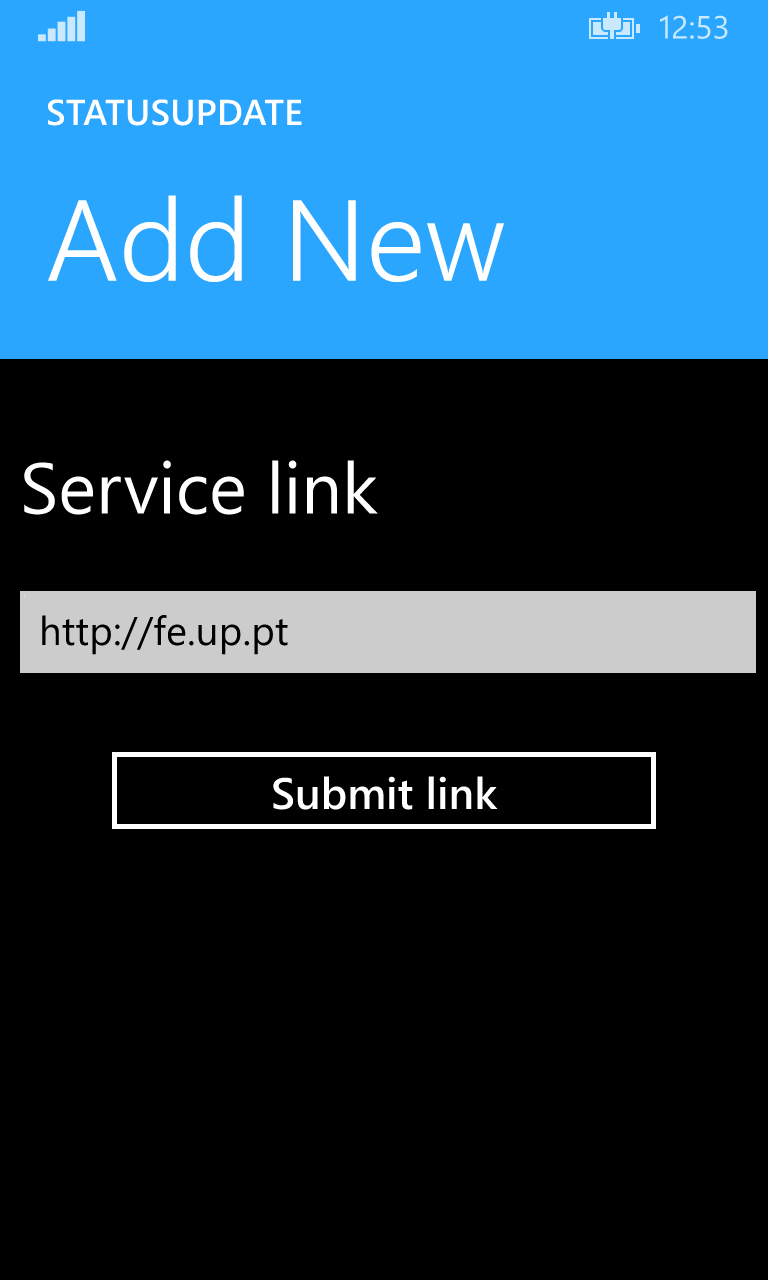
\includegraphics[width=5cm]{6.png}
\caption{Adicionar serviços.}
\label{fig:2figsB}
\end{minipage}
\end{figure}
\begin{figure}[ht!]
\centering
\parbox{5cm}{
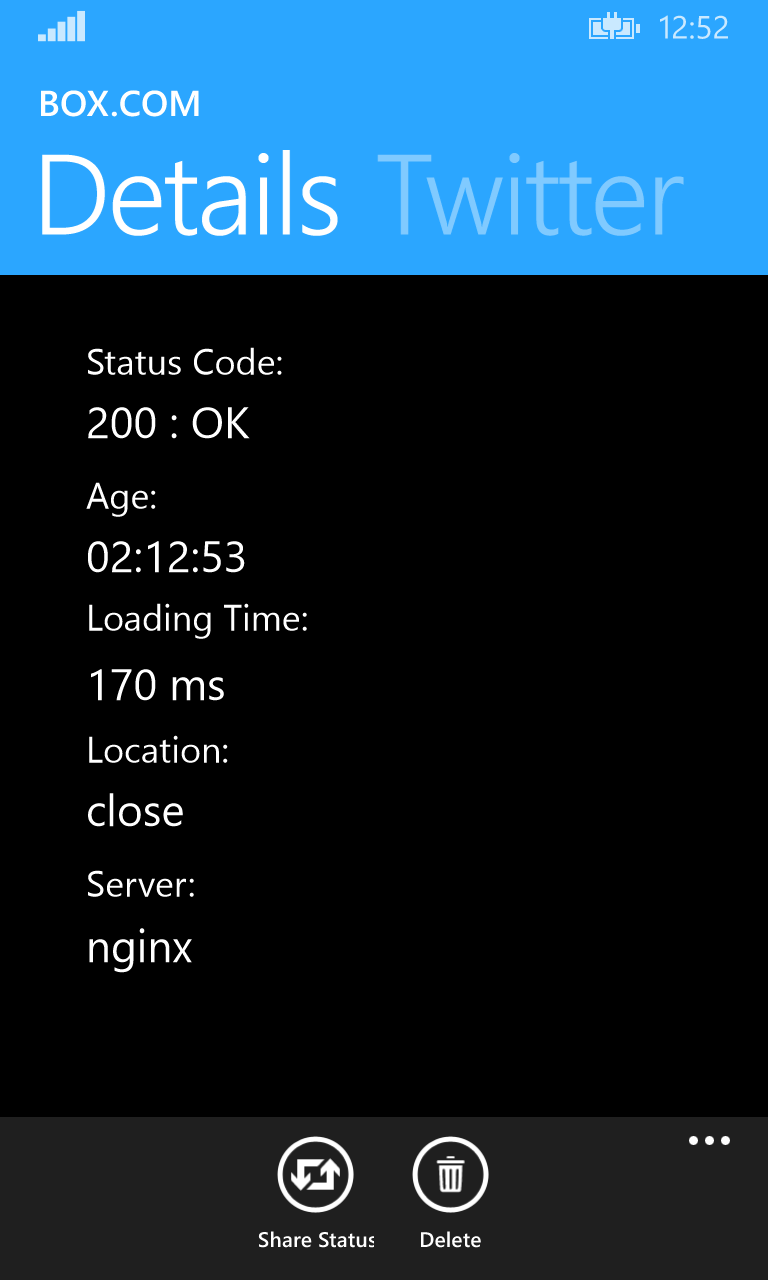
\includegraphics[width=5cm]{4.png}
\caption{Detalhes de um serviço.}
\label{fig:2figsA}}
\qquad
\begin{minipage}{5cm}
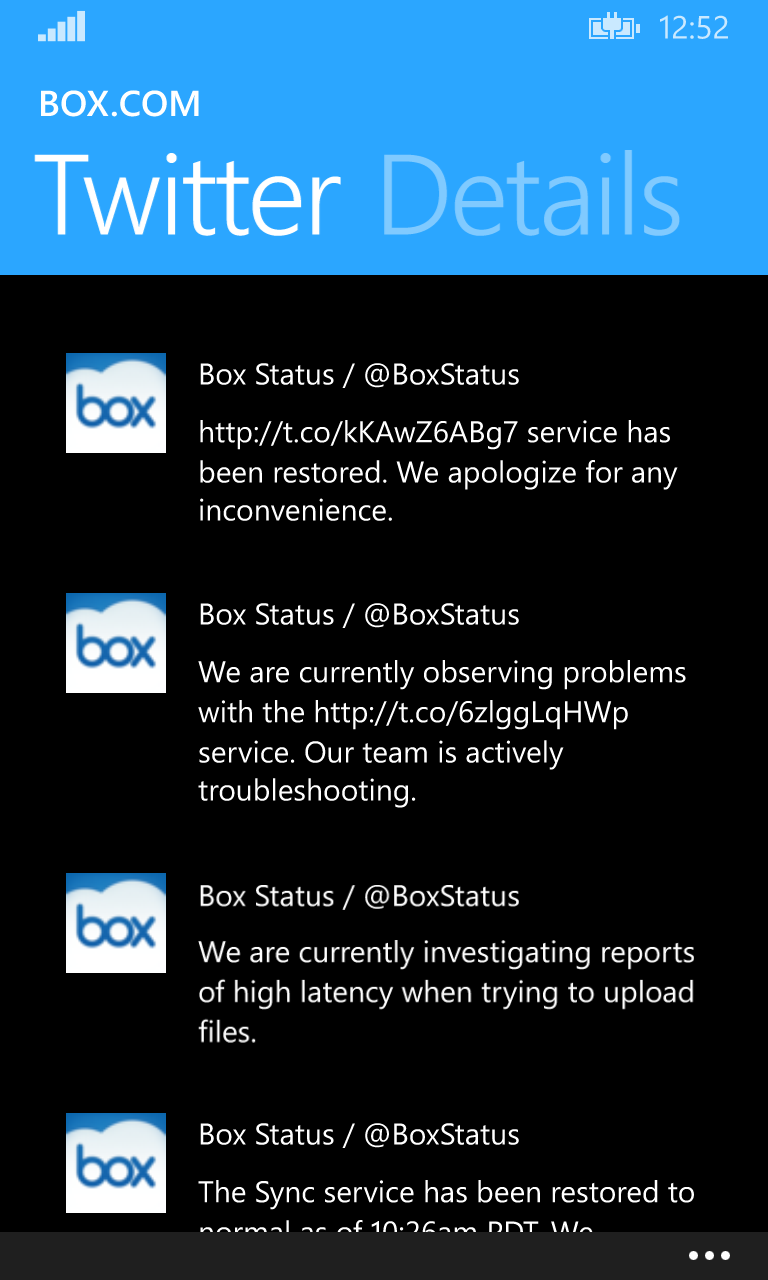
\includegraphics[width=5cm]{5.png}
\caption{Feed da conta Twitter associada ao serviço.}
\label{fig:2figsB}
\end{minipage}
\end{figure}
\newpage
\section{Conclusão}

O desenvolvimento deste projeto foi efetuado de forma gradual, implementando sempre as funcionalidades que, a nosso ver, iriam fazer falta numa utilização diária da aplicação. Assim a utilização das tecnológias escolhidas e apresentadas foi uma mais valia sendo que são tecnológias altamente escaláveis e estaveis.

A utilização de comunicação REST verificou-se que tornou toda a comunicação cliente-servidor simples e rápida que era exatamente o pretendido.

Assim criou-se uma aplicação que tem bastante utilidade no mundo atual, em que se verifica uma dependência de serviços web.

A nível da utilização da informação que foi disponibilizada ao longo da unidade curricular, verificou-se que não era suficiente para os objetivos que pretendiamos atingir, sendo que a disponibilização de informação relativa as plataformas para o lado servidor, como foi utilizado no nosso caso Node.js, e uma maior incisão na programação móvel mostrariam um elevado grau de importância. 
\begin{thebibliography}{1}

\bibitem{bl}heroku dev center, \url{https://devcenter.heroku.com/articles/getting-started-with-nodejs}, 20 05 2014.

\bibitem{b1}The MongoDB 2.6 Manual, \url{http://docs.mongodb.org/manual/},22 05 2014.

\bibitem{b2}Windows Phone Dev Center, \url{https://dev.windowsphone.com/en-us/develop}, 29 05 2014.

\end{thebibliography}


\end{document}
